\chapter{Introducción}
\pagenumbering{arabic}
Los sismos son fenómenos con los que interactuamos con bastante frecuencia \cite{Shearer2019}. Cada día, suceden aproximadamente 50 temblores perceptibles en el mundo. La ciencia que utilizamos para estudiar estos fenómenos es la sismología, esta es una ciencia moderna, que tiene sus inicios en las últimas décadas del siglo XIX, cuando Robert Mallet viajó a Nápoles para documentar la destrucción del terremoto de 1857. El trabajo de Mallet fue el primer paso para el estudio de los sismos de forma científica. \cite{Shearer2019}. Las ondas mecánicas generadas por los sismos nos ayudan a conocer la composición de las capas internas de la tierra, las cuales no podemos observar directamente. Esto se utiliza, por ejemplo, en la prospección de yacimientos petrolíferos. También, al conocer el comportamiento de las ondas generadas por temblores podemos detectar ondas artificiales, lo que da paso a la detección de pruebas nucleares \cite{Shearer2019}.

En la ciencia, el uso de simulaciones permite comparar modelos con datos observados, esto sirve para evaluar los ámbitos en los que el modelo puede ser o no válido. En la sismología, existen métodos de simulación clásicos como lo es la teoría de rayos y las soluciones modales, que siguen siendo útiles e importantes debido a que son menos costosas computacionalmente. Gracias al avance en hardware y software, se ha hecho posible la aplicación de métodos numéricos que permiten el cálculo de sismogramas sintéticos y la resolución de problemas tridimensionales \cite{Igel2016}. Las simulaciones en sismología son de gran importancia, ya que complementan los datos históricos y esto ayuda a la investigación, y a la toma de decisiones en áreas como lo es el diseño y la infraestructura. Un ejemplo de simulación es AWP-ODC, esta simulación hace uso del método numérico de diferencias finitas para resolver las ecuaciones diferenciales del modelo. Este software fue utilizado en el 2010 para simular sismos de magnitud 8 con una frecuencia de 2 Hz en el sur de California, abarcando un área de 800 km por 400 km en computadoras de petaescala \cite{Cui2010}, capaces de realizar $10^{15}$ operaciones de punto flotante de 64 bits por segundo (FLOPS).

El TOP500 es el listado de las supercomputadoras más poderosas en el mundo, este se actualiza de manera semestral desde 1993. En la \cref{fig:top500} podemos ver el rendimiento en FLOPS de la computadora número 1 en cada listado desde 1993 hasta el 2024 \cite{top500}. En el 2008, la supercomputadora RoadRunner se convirtió en la primer computadora de petaescala, desde entonces se notaba que las unidades de entrada/salida (E/S) no estaban avanzando tan rápido como las unidades de procesamiento, por lo que podrían convertirse en cuellos de botella \cite{Narayan2009}. Ya desde el 2007 el departamento de energía de los Estados Unidos (DoE) se empezó a preparar para el desarrollo de las supercomputadoras de exaescala, montando talleres para identificar los beneficios y retos que iban a traer, como lo es la E/S y los requerimientos energéticos del mantenimiento y uso de estos sistemas \cite{Messina2017}. Se han propuesto múltiples soluciones al problema de la E/S, como lo es la E/S paralela \cite{Byna2022} o el análisis y visualización in-situ \cite{akira_kageyama_approach_2014}.

\begin{figure}[ht]
  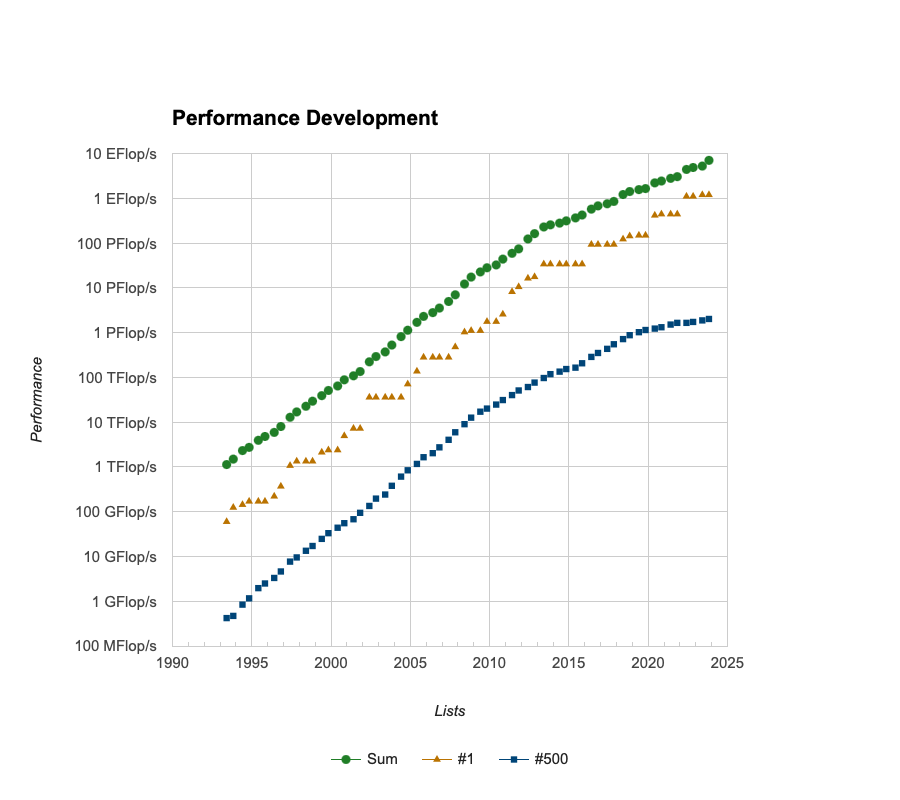
\includegraphics[width=\textwidth]{top500}
  \caption{Evolución del rendimiento de las supercomputadoras según el TOP500}
  \label{fig:top500}
\end{figure}

Tradicionalmente, el posprocesamiento de los datos de simulación se realiza una vez que esta ha finalizado de ejecutarse, lo que llamamos un procesamiento post-hoc. En contraste, el análisis y visualización in-situ se refiere a realizar el procesamiento de los datos conforme son generados. Si los datos son procesados de forma local a la simulación, se puede evitar el escribirlos al disco por lo que es posible ahorrar tiempo en la E/S del sistema. Un ejemplo de esto es una versión de AWP-ODC que fue desarrollada con capacidades de análisis in-situ por medio de la biblioteca Catalyst. Esta versión del programa demostró un rendimiento aceptable en comparación a la versión original, con la ventaja adicional de haber reducido significativamente el tamaño de almacenamiento de la salida del programa \cite{mu_-situ_2019}. Este estudio resalta los resultados prometedores y beneficiosos de utilizar bibliotecas en simulaciones numéricas de sismología para la investigación.

Otro aspecto beneficioso del análisis y visualización in-situ es la capacidad de dirigir computacionalmente las simulaciones \cite{Grosset2020}. Tradicionalmente, las visualizaciones y métricas de simulación solo estaban disponibles después de que esta haya finalizado o alcanzado un punto de control. Sin embargo, el análisis y visualización in-situ permite que los resultados estén disponibles constantemente durante la simulación, lo que brinda a los investigadores la oportunidad de tomar decisiones anticipadas, como detener la simulación si comienza a divergir o si cambian las condiciones. Este tipo de interacción con las simulaciones se ha utilizado en otros dominios \cite{Yi2014} y sería valioso para las simulaciones sísmicas.

\section{Aportes de la investigación}
Esta investigación tendrá tres aportes principales
\begin{itemize}
  \item Una caracterización de simulaciones en otras áreas de la ciencia que hagan uso de bibliotecas de análisis in-situ. Esto será valioso para futuros investigadores que vayan a implementar sistemas similares. 
  \item La creación de una simulación sísmica que haga uso del análisis y visualización in-situ, lo que permitirá que los investigadores del área puedan tener mayor control sobre la simulación, así como hacer un mejor uso de la infraestructura computacional de exaescala. 
  \item Una evaluación del rendimiento y utilidad de la herramienta creada que servirá de referencia para la consideración de investigadores que deseen hacer uso de esta. 
  
\end{itemize}

\section{Objetivos}
\subsection{Objetivo general}
Modificar una simulación sísmica para que haga uso del análisis y visualización in-situ, basado en la caracterización de simulaciones en otros dominios de forma que sea útil, eficiente e introspectiva para el investigador.
\subsection{Objetivos específicos}
\begin{enumerate}
  \item Caracterizar simulaciones en otros dominios que hayan incorporado el análisis in-situ. % Explicar que esto terminará en un artículo.
  \item Extender una simulación sísmica numérica para que utilice el análisis y la visualización in-situ. % Explicar que esto incluye el diseño y mejora del rendimiento del programa.
  \item Estudiar el rendimiento y validar la utilidad de la simulación extendida. % Explicar que esto incluirá el criterio de expertos en el área.
\end{enumerate}
\section{Estructura}
En el \cref{chap:marco} se dará una explicación de alto nivel de las simulaciones sísmicas y se hablará de algunas que existen, así como la que se escogida para llevar a cabo la investigación. Adicionalmente se explicará el concepto de análisis y visualización in-situ y se darán ejemplos de bibliotecas existentes.
En el \cref{chap:antecedentes} se hablará de simulaciones sísmicas que hayan hecho uso del análisis in-situ y la forma en que nuestra propuesta difiere de estas, y en el \cref{chap:metodologia} se hará una exposición de la metodología que se utilizará para llevar a cabo la investigación.

% \section{Preguntas de investigación}
% ¿Cómo desarrollar una extensión usable, eficiente e introespectiva para una simulación sísmica numérica que utilice el análisis y visualización in-situ?

